\begin{table}[H]\centering\small
\caption{Participant flow (STROBE).}\label{tab:flow}
\begin{tabular}{llr}
\toprule
Cohort & Step & $n$ \\
\midrule
METABRIC & records & 2509 \\
METABRIC & invasive carcinoma, female (excl. stage 0 / sarcoma) & 2484 \\
METABRIC & analysis set (grade 1-3 recorded) & 2386 \\
MSK-2018 & samples & 1918 \\
MSK-2018 & patients & 1756 \\
MSK-2018 & female & 1746 \\
MSK-2018 & analysis set (grade 1-3 recorded) & 1573 \\
MBCproject & patients & 301 \\
MBCproject & female, abstraction complete & 256 \\
MBCproject & invasive carcinoma & 254 \\
MBCproject & analysis set (grade 1-3 recorded) & 207 \\
Sanger & patients & 100 \\
Sanger & analysis set (grade 1-3 recorded) & 100 \\
Broad (MX/VN) & patients & 103 \\
Broad (MX/VN) & invasive carcinoma & 94 \\
Broad (MX/VN) & analysis set (grade 1-3 recorded) & 59 \\
BCCRC (TNBC) & patients & 65 \\
BCCRC (TNBC) & carcinoma & 64 \\
BCCRC (TNBC) & analysis set (grade 1-3 recorded) & 63 \\
Duke MRI & patients & 922 \\
Duke MRI & invasive carcinoma & 921 \\
Duke MRI & analysis set (grade 1-3 recorded) & 637 \\
TCGA-BRCA & patients & 1084 \\
TCGA-BRCA & female & 1072 \\
\bottomrule
\end{tabular}
\end{table}

\begin{table}[H]\centering\small
\caption{Leave-one-dataset-out validation (core feature set).}\label{tab:lodo}
\tabfit{\begin{tabular}{llrrrr}
\toprule
Held-out cohort & Model & $n$ & Macro-AUC (95\% CI) & G3-AUC (95\% CI) & Macro-F1 \\
\midrule
METABRIC & Multinomial LR & 2386 & 0.698 (0.679--0.716) & 0.727 (0.706--0.747) & 0.393 \\
METABRIC & Ordinal LR (prop. odds) & 2386 & 0.696 (0.678--0.713) & 0.728 (0.707--0.748) & 0.413 \\
METABRIC & Random forest & 2386 & 0.702 (0.683--0.720) & 0.730 (0.709--0.749) & 0.410 \\
METABRIC & XGBoost & 2386 & 0.700 (0.681--0.718) & 0.725 (0.704--0.745) & 0.412 \\
METABRIC & LightGBM & 2386 & 0.689 (0.671--0.706) & 0.724 (0.704--0.745) & 0.433 \\
\addlinespace
MSK-2018 & Multinomial LR & 1573 & 0.659 (0.632--0.685) & 0.684 (0.657--0.711) & 0.285 \\
MSK-2018 & Ordinal LR (prop. odds) & 1573 & 0.670 (0.645--0.695) & 0.681 (0.654--0.709) & 0.257 \\
MSK-2018 & Random forest & 1573 & 0.664 (0.638--0.691) & 0.676 (0.649--0.703) & 0.302 \\
MSK-2018 & XGBoost & 1573 & 0.662 (0.635--0.689) & 0.672 (0.645--0.700) & 0.315 \\
MSK-2018 & LightGBM & 1573 & 0.661 (0.634--0.688) & 0.673 (0.645--0.700) & 0.335 \\
\addlinespace
MBCproject & Multinomial LR & 207 & 0.709 (0.656--0.759) & 0.778 (0.713--0.840) & 0.322 \\
MBCproject & Ordinal LR (prop. odds) & 207 & 0.716 (0.665--0.763) & 0.771 (0.706--0.835) & 0.483 \\
MBCproject & Random forest & 207 & 0.707 (0.658--0.756) & 0.770 (0.703--0.835) & 0.332 \\
MBCproject & XGBoost & 207 & 0.710 (0.658--0.760) & 0.773 (0.705--0.839) & 0.358 \\
MBCproject & LightGBM & 207 & 0.714 (0.664--0.764) & 0.764 (0.697--0.831) & 0.329 \\
\addlinespace
Sanger & Multinomial LR & 100 & 0.778 (0.692--0.855) & 0.787 (0.692--0.871) & 0.483 \\
Sanger & Ordinal LR (prop. odds) & 100 & 0.759 (0.675--0.838) & 0.791 (0.696--0.871) & 0.464 \\
Sanger & Random forest & 100 & 0.769 (0.683--0.847) & 0.786 (0.690--0.869) & 0.391 \\
Sanger & XGBoost & 100 & 0.774 (0.683--0.857) & 0.791 (0.695--0.875) & 0.442 \\
Sanger & LightGBM & 100 & 0.761 (0.670--0.845) & 0.791 (0.695--0.874) & 0.455 \\
\addlinespace
Duke MRI & Multinomial LR & 637 & 0.703 (0.676--0.730) & 0.782 (0.743--0.820) & 0.459 \\
Duke MRI & Ordinal LR (prop. odds) & 637 & 0.705 (0.678--0.732) & 0.782 (0.744--0.820) & 0.465 \\
Duke MRI & Random forest & 637 & 0.717 (0.688--0.744) & 0.787 (0.749--0.825) & 0.460 \\
Duke MRI & XGBoost & 637 & 0.712 (0.682--0.739) & 0.782 (0.743--0.822) & 0.446 \\
Duke MRI & LightGBM & 637 & 0.708 (0.678--0.736) & 0.780 (0.741--0.819) & 0.458 \\
\bottomrule
\end{tabular}}
\end{table}

\begin{table}[H]\centering\small
\caption{Calibration of P(grade 3): intercept (calibration-in-the-large) and slope, internally, in
the external full-feature cohorts and after a cross-fitted intercept update.}\label{tab:cal}
\tabfit{\begin{tabular}{llrrrrrr}
\toprule
Model & Setting & $n$ & Obs. G3 & Mean pred. & Intercept & Slope & G3-AUC \\
\midrule
Multinomial LR & METABRIC (internal CV) & 2386 & 0.502 & 0.502 & -0.00 & 1.00 & 0.753 \\
Multinomial LR & MSK-2018 (external) & 1573 & 0.676 & 0.472 & +0.99 & 1.03 & 0.727 \\
Multinomial LR & MSK-2018 (intercept-updated) & 1573 & 0.676 & 0.676 & +0.00 & 1.03 & 0.727 \\
Multinomial LR & Duke MRI (external) & 637 & 0.325 & 0.517 & -1.02 & 0.96 & 0.779 \\
Multinomial LR & Duke MRI (intercept-updated) & 637 & 0.325 & 0.325 & +0.00 & 0.96 & 0.779 \\
Ordinal LR (prop. odds) & METABRIC (internal CV) & 2386 & 0.502 & 0.501 & +0.00 & 0.96 & 0.752 \\
Ordinal LR (prop. odds) & MSK-2018 (external) & 1573 & 0.676 & 0.474 & +0.97 & 1.02 & 0.725 \\
Ordinal LR (prop. odds) & MSK-2018 (intercept-updated) & 1573 & 0.676 & 0.676 & +0.00 & 1.02 & 0.724 \\
Ordinal LR (prop. odds) & Duke MRI (external) & 637 & 0.325 & 0.520 & -1.05 & 0.92 & 0.778 \\
Ordinal LR (prop. odds) & Duke MRI (intercept-updated) & 637 & 0.325 & 0.325 & +0.00 & 0.92 & 0.777 \\
XGBoost & METABRIC (internal CV) & 2386 & 0.502 & 0.503 & -0.00 & 1.02 & 0.755 \\
XGBoost & MSK-2018 (external) & 1573 & 0.676 & 0.474 & +0.98 & 1.03 & 0.726 \\
XGBoost & MSK-2018 (intercept-updated) & 1573 & 0.676 & 0.676 & +0.00 & 1.03 & 0.726 \\
XGBoost & Duke MRI (external) & 637 & 0.325 & 0.519 & -1.06 & 0.97 & 0.789 \\
XGBoost & Duke MRI (intercept-updated) & 637 & 0.325 & 0.325 & -0.00 & 0.97 & 0.789 \\
\bottomrule
\end{tabular}}
\end{table}

\begin{table}[H]\centering\small
\caption{Multiclass calibration-in-the-large: observed versus mean predicted prevalence of each grade (\%).}\label{tab:oe}
\tabfit{\begin{tabular}{llrrrrrr}
\toprule
Model & Setting & Obs. G1 & Pred. G1 & Obs. G2 & Pred. G2 & Obs. G3 & Pred. G3 \\
\midrule
Multinomial LR & METABRIC (internal CV) & 8.9 & 8.9 & 40.9 & 40.9 & 50.2 & 50.2 \\
Multinomial LR & MSK-2018 (external) & 5.7 & 8.5 & 26.7 & 44.3 & 67.6 & 47.2 \\
Multinomial LR & Duke MRI (external) & 17.7 & 7.6 & 49.8 & 40.7 & 32.5 & 51.7 \\
Ordinal LR (prop. odds) & METABRIC (internal CV) & 8.9 & 9.0 & 40.9 & 40.9 & 50.2 & 50.1 \\
Ordinal LR (prop. odds) & MSK-2018 (external) & 5.7 & 9.1 & 26.7 & 43.5 & 67.6 & 47.4 \\
Ordinal LR (prop. odds) & Duke MRI (external) & 17.7 & 8.1 & 49.8 & 39.9 & 32.5 & 52.0 \\
XGBoost & METABRIC (internal CV) & 8.9 & 8.9 & 40.9 & 40.8 & 50.2 & 50.3 \\
XGBoost & MSK-2018 (external) & 5.7 & 8.7 & 26.7 & 43.8 & 67.6 & 47.4 \\
XGBoost & Duke MRI (external) & 17.7 & 8.2 & 49.8 & 39.9 & 32.5 & 51.9 \\
\bottomrule
\end{tabular}}
\end{table}

\begin{table}[H]\centering\small
\caption{Missing data: multiple imputation with pooled predictions and complete-case analysis versus
the primary single in-fold imputation (METABRIC, nested cross-validation).}\label{tab:mi}
\tabfit{\begin{tabular}{llrrrrr}
\toprule
Model & Missing-data method & $n$ & Macro-AUC (95\% CI) & G3-AUC & Macro-F1 & Brier \\
\midrule
Multinomial LR & Multiple imputation (m=20, pooled predictions) & 2386 & 0.724 (0.707--0.742) & 0.752 & 0.465 & 0.490 \\
Multinomial LR & Complete-case analysis & 1800 & 0.729 (0.709--0.747) & 0.761 & 0.455 & 0.486 \\
Multinomial LR & Single in-fold imputation (primary) & 2386 & 0.725 (0.707--0.742) & 0.752 & 0.465 & 0.490 \\
XGBoost & Multiple imputation (m=20, pooled predictions) & 2386 & 0.726 (0.710--0.745) & 0.755 & 0.465 & 0.489 \\
XGBoost & Complete-case analysis & 1800 & 0.727 (0.709--0.747) & 0.760 & 0.453 & 0.487 \\
XGBoost & Single in-fold imputation (primary) & 2386 & 0.723 (0.708--0.743) & 0.753 & 0.458 & 0.492 \\
\bottomrule
\end{tabular}}
\end{table}

\begin{table}[H]\centering\small
\caption{Minimum sample size for developing the multinomial model (Riley criteria applied to each
pairwise sub-model).}\label{tab:ss}
\tabfit{\begin{tabular}{lrrrrr}
\toprule
Sub-model & Share of patients & Anticipated $R^2_{CS}$ & Max $R^2_{CS}$ & $n$ (criterion i) & $n$ (criterion ii) \\
\midrule
G1 vs G2 & 0.498 & 0.039 & 0.610 & 4477 & 636 \\
G1 vs G3 & 0.591 & 0.180 & 0.572 & 758 & 528 \\
G2 vs G3 & 0.911 & 0.171 & 0.747 & 521 & 263 \\
\midrule
Criterion (iii): each grade prevalence $\pm$0.05 & & & & \multicolumn{2}{r}{385} \\
Required (maximum) / available & & & & \multicolumn{2}{r}{4477 / 2386} \\
\bottomrule
\end{tabular}}
\end{table}

\begin{table}[H]\centering\small
\caption{Sensitivity of the Saudi-weighted METABRIC grade distribution (\%) to the assumed share of
patients aged $\le$50 years in the Dammam series (which reports only the median age).}\label{tab:agesens}
\begin{tabular}{rrrrr}
\toprule
Assumed share $\le$50 y & ESS & G1 & G2 & G3 \\
\midrule
40\% & 1278 & 6.3 & 33.2 & 60.5 \\
45\% & 1187 & 6.3 & 33.0 & 60.7 \\
50\% & 1088 & 6.2 & 32.9 & 60.9 \\
55\% & 988 & 6.2 & 32.7 & 61.1 \\
60\% & 892 & 6.1 & 32.6 & 61.3 \\
\bottomrule
\end{tabular}
\end{table}

\begin{table}[H]\centering\small
\caption{Ljubljana sensitivity analysis (``degree of malignancy''; age band, menopausal status,
tumour-size band, nodes, node capsule invasion; \Repeats$\times$5-fold CV).}\label{tab:lj}
\tabfit{\begin{tabular}{lrrrr}
\toprule
Model & $n$ & Macro-AUC (SD over repeats) & Macro-F1 & G3-AUC \\
\midrule
Majority class & 286 & 0.497 (0.000) & 0.208 & 0.498 \\
Multinomial LR & 286 & 0.636 (0.011) & 0.425 & 0.691 \\
Ordinal LR (prop. odds) & 286 & 0.618 (0.010) & 0.397 & 0.694 \\
Random forest & 286 & 0.626 (0.018) & 0.392 & 0.698 \\
XGBoost & 286 & 0.622 (0.014) & 0.402 & 0.686 \\
\bottomrule
\end{tabular}}
\end{table}

\begin{figure}[H]\centering
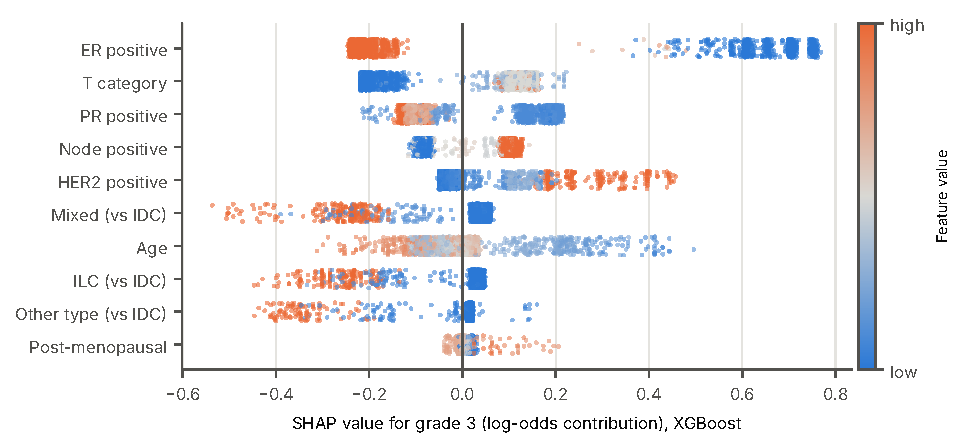
\includegraphics[width=0.86\linewidth]{generated/fig_shap.pdf}
\caption{SHAP beeswarm for the grade-3 output of XGBoost in METABRIC; colour encodes the (imputed)
feature value.}\label{fig:beeswarm}
\end{figure}

\small
% Full TRIPOD+AI checklist (Collins et al., BMJ 2024; 27 main-text items). D = development, E = evaluation.
\begin{longtable}{p{0.6cm}p{3.0cm}p{0.8cm}p{7.5cm}}
\caption{TRIPOD+AI checklist: where each item is reported.}\label{tab:tripod}\\
\toprule
Item & Topic & D/E & Location in this paper \\
\midrule\endfirsthead
\toprule Item & Topic & D/E & Location \\ \midrule\endhead
\bottomrule\endfoot
1 & Title & D;E & Title: prediction of grade, development and external validation, open data \\
2 & Abstract & D;E & Structured abstract (TRIPOD+AI for Abstracts items) \\
3a & Background: healthcare context & D;E & Introduction, paragraphs 1 and 3 \\
3b & Background: target population and intended use & D;E & Introduction, paragraph 1 (baseline for image models, registry imputation, quality assurance); Discussion, \emph{Implications} \\
3c & Background: known biases/inequalities & D;E & Introduction, paragraph 3 (Saudi/Gulf case-mix, absence of open regional data) \\
4 & Objectives & D;E & Introduction, \emph{Contributions} \\
5a & Data sources & D;E & Methods, \emph{Data sources}; Table~\ref{tab:cohorts} \\
5b & Dates of data collection & D;E & Methods, \emph{Data sources}; Supplementary Table~\ref{tab:flow}; Data availability (download date and checksums) \\
6a & Setting and centres & D;E & Methods, \emph{Data sources} \\
6b & Eligibility criteria & D;E & Methods, \emph{Harmonisation} (rules i--iv) \\
6c & Treatments received & D;E & Not applicable at diagnosis (grade is a baseline characteristic); Limitations \\
7 & Data preparation & D;E & Methods, \emph{Harmonisation}; repository \texttt{harmonise.py} \\
8a & Outcome definition & D;E & Methods, \emph{Outcome}: invasive Nottingham grade 1--3; grade 3 vs 1--2 \\
8b & Outcome assessment & D;E & Assigned by pathologists at each source; differences discussed under Limitations \\
8c & Blinding of outcome assessment & D;E & Not applicable (retrospective records); Limitations \\
9a & Choice of predictors & D & Methods, \emph{Outcome, predictors and feature sets} \\
9b & Predictor definitions & D;E & Methods, \emph{Harmonisation}; repository code \\
9c & Blinding of predictor assessment & D;E & Not applicable (routine records); leakage quarantine \\
10 & Sample size & D;E & Methods, \emph{Sample size}; Supplementary Table~\ref{tab:ss} \\
11 & Missing data & D;E & Methods, \emph{Missing data}; Supplementary Table~\ref{tab:mi} \\
12a & Data use (development/evaluation) & D;E & Methods, \emph{Validation}; Figure~\ref{fig:framework} \\
12b & Pre-processing & D & Methods, \emph{Model development} (in-fold imputation and scaling) \\
12c & Model type and building & D & Methods, \emph{Model development} \\
12d & Heterogeneity across clusters & D;E & LODO validation; cohort-level results (Tables~\ref{tab:external}, \ref{tab:lodo}) \\
12e & Performance measures & D;E & Methods, \emph{Performance measures} \\
12f & Model updating & E & Methods, \emph{Performance measures} (intercept update) \\
12g & Comparison with other models & D;E & Model ladder; paired $\Delta$ vs LR (Table~\ref{tab:internal}) \\
13 & Class imbalance & D;E & Methods, \emph{Model development} (no resampling; prevalence-adjusted rule) \\
14 & Fairness & D;E & Results by country/cohort; Saudi transport (Section~\ref{sec:transport}) \\
15 & Model output & D & Probabilities for each grade \\
16 & Training versus evaluation differences & D;E & Methods, \emph{Validation}; frozen external models \\
17 & Ethical approval & D;E & Declarations \\
18a & Funding & D;E & Declarations \\
18b & Conflicts of interest & D;E & Declarations \\
18c & Protocol & D;E & Pre-specified analysis plan in \texttt{configs/experiment.yaml} (repository) \\
18d & Registration & D;E & Not registered (secondary analysis of open data); Declarations \\
18e & Data sharing & D;E & Data availability \\
18f & Code sharing & D;E & Code availability \\
19 & Patient and public involvement & D;E & Declarations \\
20a & Participant flow & D;E & Supplementary Table~\ref{tab:flow} \\
20b & Participant characteristics & D;E & Table~\ref{tab:cohorts}; Figure~\ref{fig:grade} \\
20c & Comparison of development and evaluation data & E & Table~\ref{tab:cohorts}; Results, \emph{Cohorts} \\
21 & Number of participants and outcome events & D;E & Tables~\ref{tab:cohorts}, \ref{tab:internal}, \ref{tab:external} \\
22 & Full model specification & D & Code and fitted coefficients in the repository; ordinal odds ratios (Table~\ref{tab:shap}) \\
23a & Performance with CIs & D;E & Tables~\ref{tab:internal}, \ref{tab:external}; Figure~\ref{fig:ladder} \\
23b & Performance in subgroups & D;E & By cohort/country; Saudi-weighted performance (Table~\ref{tab:transport}) \\
24 & Model updating results & E & Figure~\ref{fig:cal}; Supplementary Table~\ref{tab:cal} \\
25 & Interpretation & D;E & Discussion, \emph{Principal findings} \\
26 & Limitations & D;E & Discussion, \emph{Strengths and limitations} \\
27a & Usability: handling poor-quality or missing input & D & Methods, \emph{Missing data}; Discussion \\
27b & Usability: user interaction and expertise & D & Discussion, \emph{Implications} \\
27c & Next steps and generalisability & D;E & Discussion, \emph{Implications and next steps} \\
\end{longtable}

\normalsize
